\chapter{PERANCANGAN SISTEM}

\section{Desain Sistem}
\begin{figure}[H]
	\centering
	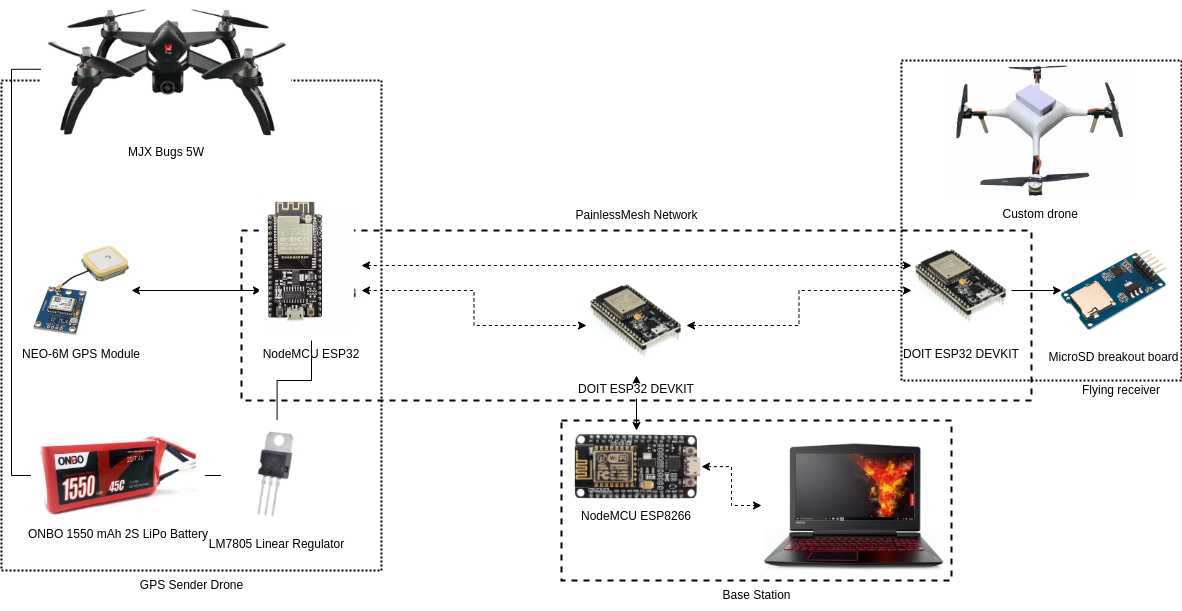
\includegraphics[scale=0.35]{./assets/DiagramHWNewV2}
	\caption{Diagram implementasi sistem.}
\end{figure}
Desain dan implementasi tugas akhir ini bertujuan untuk merancang sebuah sistem algoritma komunikasi antar-UAV menggunakan jaringan mesh berbasis ESP32. Perancangan sistem terdiri dari proses perancangan blok diagram sistem, penjelasan sistem secara umum, perancangan perangkat keras sistem, serta perancangan dan penjelasan perangkat lunak sistem yang meliputi algoritma komunikasi tersebut.

\subsection{Prinsip Kerja Sistem}
Berdasarkan rumusan masalah yang telah dipaparkan pada bab 1, berikut adalah konsep prinsip kerja sistem yang dikembangkan:
\begin{enumerate}
	\item Terdapat 2 drone dan 1 \textit{Base Station} (BS), masing-masing menggunakan mikrokontroler ESP32 yang berkomunikasi satu sama lain menggunakan JSON \textit{messages} pada jaringan PainlessMesh. Drone 1 disebut sebagai \textit{"sender node"}, dan drone 2 disebut sebagai \textit{"receiver node"}.
	\item ESP32 Drone 1 mengaktifkan modul GPS dan mendata koordinat lokasi, ketinggian terbang drone, dan jumlah satelit yang mendapat \textit{lock}, kemudian menghidupkan LED hijau pada \textit{board}.
	\item Drone 2 mengirimkan permintaan data lokasi kepada drone 1.
	\item Drone 1 mengirimkan data melalui jaringan mesh kepada drone 2. Drone 2 menghidupkan LED hijau setelah menerima data lokasi yang valid.
	\item BS mengirimkan permintaan data pada drone 1 berupa \textit{string} dalam \textit{message}.
	\item Drone 1 mengirimkan data melalui jaringan mesh kepada BS.
	\item BS menampilkan data kepada pengguna melalui \textit{WiFi Access Point} yang dapat diakses dari sebuah \textit{website}. WiFi AP tersebut dibangun menggunakan sebuah board ESP8266 yang menerima data dari board ESP32 yang terhubung dengan jaringan mesh melalui sambungan serial.
\end{enumerate}

\subsection{Diagram Blok}
\begin{figure}[H]
	\centering
	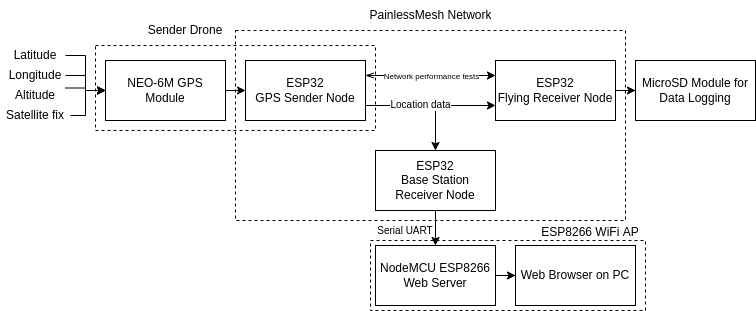
\includegraphics[scale=0.5]{./assets/DiagramBlokTANew}
	\caption{Diagram blok sistem.}
\end{figure}

Gambar 3.1 merupakan diagram blok dari sistem yang dirancang. Secara keseluruhan, sistem dapat dibagi menjadi 3 bagian, yakni \textbf{\textit{Sender}}, \textbf{\textit{Flying Receiver}}, dan \textbf{\textit{Base Station Receiver}}.
\subsubsection{Sender Node}
Sender node merupakan board ESP32 yang diterbangkan menggunakan drone \textit{Victim Finder} dan bertugas menerima data lokasi dari modul GPS dan kemudian mengirimkan data lokasi tersebut berdasarkan permintaan dari \textit{receiver}. Board ESP32 mendapatkan data lokasi dari modul GPS dengan menggunakan komunikasi serial UART pada baud rate 9600, yang kemudian modul GPS mengirimkan data lokasi berupa kalimat-kalimat NMEA. Data tersebut kemudian diolah menggunakan library TinyGPS++ untuk memudahkan penafsiran kalimat-kalimat NMEA tersebut.

Karena sistem \textit{messaging} di PainlessMesh menggunakan JSON, maka data lokasi yang telah didapatkan (lintang, bujur, ketinggian, dan jumlah satelit yang sudah \textit{lock}) dikirimkan berupa JSON \textit{values} dengan \textit{key} berupa \textit{latitude, longitude, altitude,} dan \textit{satellite}. Data JSON tersebut dihitung besarnya dalam byte untuk kepentingan pengukuran \textit{throughput}, kemudian ditambahkan \textit{timestamp} pengiriman.

\subsubsection{Flying Receiver Node}
Receiver node ini merupakan board ESP32 yang dilengkapi board MicroSD untuk kepentingan \textit{data logging}. Board ini akan diterbangkan oleh sebuah drone dan bertugas melakukan permintaan data lokasi kepada node Sender, sekaligus melakukan pengujian kinerja jaringan, yakni pengujian \textit{throughput}, pengujian \textit{packet loss}, dan pengujian \textit{round-trip delay}. Hasil dari pengujian tersebut kemudian disimpan dalam sebuah kartu microSD untuk diolah dan dianalisis.

\subsubsection{Base Station Receiver Node}
Receiver node ini merupakan board ESP32 yang disambungkan secara serial dengan sebuah board ESP8266 yang bertugas menjadi web server untuk menampilkan data lokasi pada sebuah situs web. Konfigurasi ini diperlukan karena keterbatasan pengujian, dimana mode 802.11LR pada ESP32 merupakan mode \textit{proprietary} yang tidak didukung oleh piranti WiFi lainnya, serta jaringan PainlessMesh yang membutuhkan mode AP dari ESP32, sedangkan board ESP32 hanya mendukung maksimal 1 AP per board. Oleh karena itu, dibutuhkan satu board lain untuk menjadi web server.

\subsection{Fungsi dan Fitur}
Sistem yang dirancang untuk tugas akhir ini memiliki fungsi komunikasi data lokasi dari satu drone kepada drone lain dan \textit{base station}. Karena posisi antar drone dan \textit{base station} yang bervariasi serta target penggunaan di daerah tanpa infrastruktur, maka dibutuhkan metode komunikasi yang fleksibel terhadap disrupsi dan tidak bergantung pada infrastruktur yang sudah ada, oleh karena itu digunakan sebuah jaringan mesh menggunakan PainlessMesh sehingga komunikasi dapat terjalin pada jaringan yang mampu melakukan \textit{self-healing} dan \textit{autoconfiguration} ketika terjadi disrupsi.

\section{Desain Perangkat Keras}
Perangkat yang digunakan pada sistem ini adalah tiga buah board DOIT ESP32 Development Kit, sebuah board NodeMCU ESP8266, sebuah modul GPS NEO-6M, sebuah board modul MicroSD, baterai Lithium-Polymer (LiPo) 2S 1500 mAh, sebuah linear regulator LM7805, dan dua buah drone. Sistem dapat menerima daya dari baterai LiPo melalui konektor \textit{balance} JST XH, yang kemudian tegangannya diturunkan menggunakan linear regulator LM7805 ke tegangan 5V.

Perancangan sistem membutuhkan komponen-komponen pendukung untuk dapat merealisasikan sistem, diantaranya adalah board DOIT-ESP32-DEVKIT, modul GPS NEO-6M, drone MJX Bugs 5W, dan \textit{power supply}, dengan spesifikasi sebagai berikut:
\begin{enumerate}
	\item Ai-Thinker NodeMCU-32S\newline Board Ai-Thinker NodeMCU-32S adalah sebuah \textit{development kit} berbasis mikrokontroler ESP32S dari Ai-Thinker. Board ini memiliki kapabilitas Wi-Fi dan Bluetooth, serta mendukung penggunaan antena eksternal melalui konektor Hirose U.FL. Menggunakan kabel \textit{pigtail} konverter U.FL ke konektor SubMiniature A (SMA), maka board ini dapat dengan mudah dihubungkan dengan sebuah antena eksternal 2.4 GHz. Pada perancangan sistem ini, board ini digunakan sebagai modul komunikasi pada drone \textit{sender}.
	\begin{figure}[H]
		\centering
		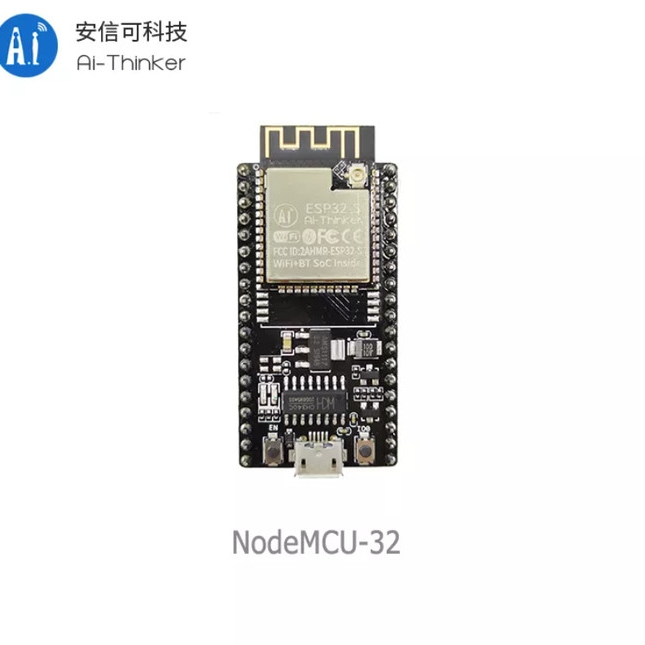
\includegraphics[scale=0.4]{./assets/NodeMCU32}
		\caption{Board Ai-Thinker NodeMCU-32S}
	\end{figure}
	\captionof{table}{Spesifikasi Ai-Thinker NodeMCU-32S}
	\begin{longtable}{|p{2cm}|p{8cm}|}
		\hline
		SOC&2x Xtensa 32-bit LX6 microprocessor up to 240MHz, 384KB ROM, 512KB SRAM\\
		\hline
		Konektivitas&WiFi 802.11 (B/G/N/LR), Bluetooth LE\\
		\hline
		IO&18 channel ADC, 10 capacitive sensing GPIO, 3 UART interfaces, 3 SPI interfaces, 2 I$^2$C interfaces, 16 PWM output channels, 2 channel DAC, 2 I$^2$S interfaces\\
		\hline
		Masukan tegangan&5V regulated, 6V - 20V unregulated\\
		\hline
		Tegangan operasional&3.3V\\
		\hline
		Temperatur operasi&-40\textdegree C - 85\textdegree C\\
		\hline
	\end{longtable}

	\item DOIT-ESP32-DEVKIT\newline Board DOIT-ESP32-DEVKIT adalah sebuah \textit{development kit} yang menggunakan mikrokontroler ESP32, sehingga memiliki kapabilitas Wi-Fi dan Bluetooth. Pada perancangan sistem ini, ESP32 digunakan sebagai modul komunikasi pada drone \textit{flying receiver} dan \textit{base station}.
	\begin{figure}[H]
		\centering
		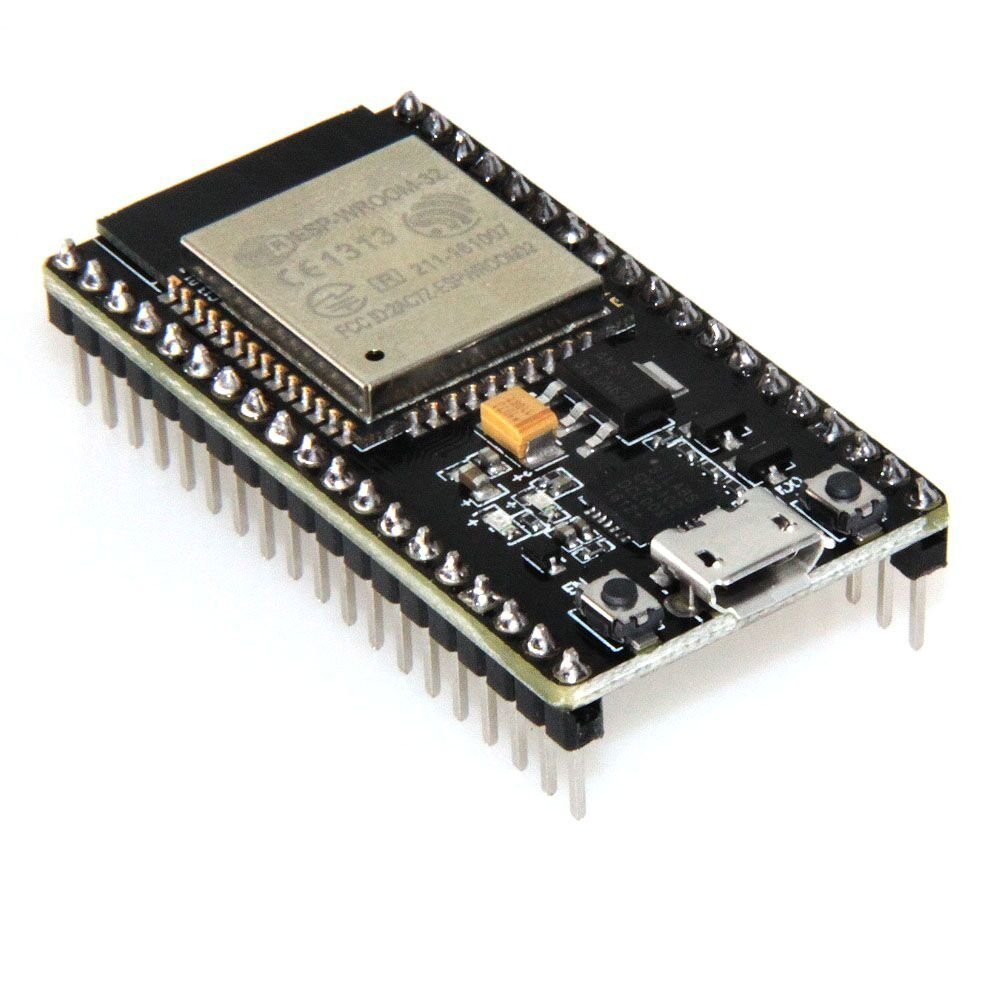
\includegraphics[scale=0.2]{./assets/ESP32}
		\caption{Board DOIT-ESP32-DEVKIT}
	\end{figure}
	\captionof{table}{Spesifikasi DOIT-ESP32-DEVKIT}
	\begin{longtable}{|p{2cm}|p{8cm}|}
		\hline
		SOC&2x Xtensa 32-bit LX6 microprocessor up to 240MHz, 448KB ROM, 520KB SRAM\\
		\hline
		Konektivitas&WiFi 802.11 (B/G/N/LR), Bluetooth\\
		\hline
		IO&18 channel ADC, 10 capacitive sensing GPIO, 3 UART interfaces, 3 SPI interfaces, 2 I$^2$C interfaces, 16 PWM output channels, 2 channel DAC, 2 I$^2$S interfaces\\
		\hline
		Masukan tegangan&5V regulated, 6V - 20V unregulated\\
		\hline
		Tegangan operasional&3.3V\\
		\hline
		Temperatur operasi&-40\textdegree C - 85\textdegree C\\
		\hline
	\end{longtable}
	
	\item Ai-Thinker NodeMCU ESP-12S (ESP8266)\newline Board Ai-Thinker NodeMCU ESP-12S adalah sebuah \textit{development kit} yang menggunakan mikrokontroler ESP8266. Pada perancangan sistem ini, ESP8266 digunakan sebagai \textit{web server} yang menampilkan data lokasi drone sender yang diterima oleh \textit{base station} ESP32 melalui UART.
	\begin{figure}[H]
		\centering
		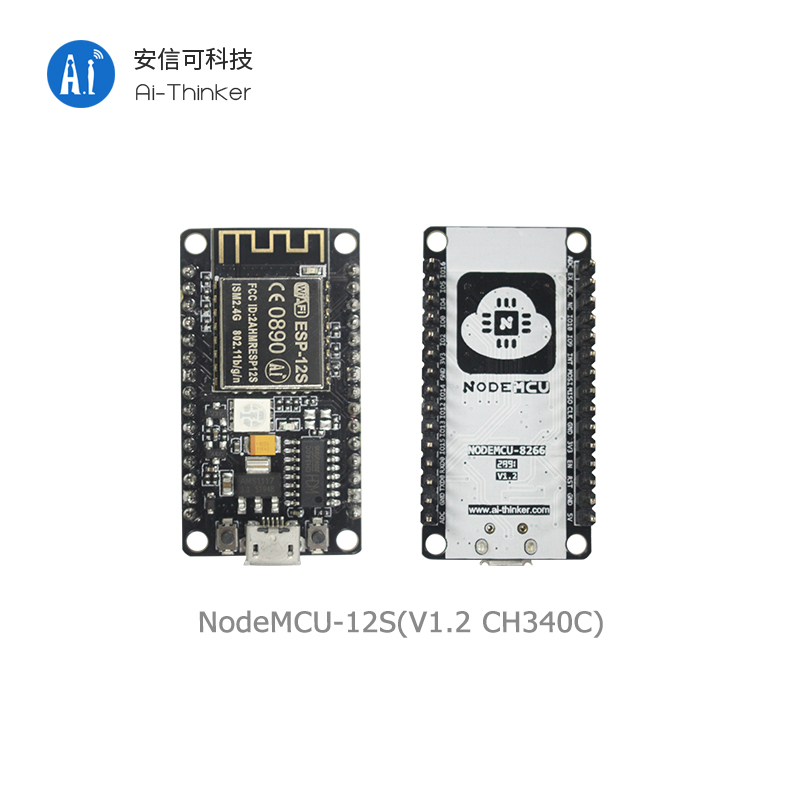
\includegraphics[scale=0.4]{./assets/NodeMCU8266}
		\caption{Board Ai-Thinker NodeMCU ESP-12S}
	\end{figure}
	\captionof{table}{Spesifikasi Ai-Thinker NodeMCU ESP-12S}
	\begin{longtable}{|p{2cm}|p{8cm}|}
		\hline
		SOC&Tensilica L106 32-bit 160 MHz\\
		\hline
		Konektivitas&WiFi 802.11 (B/G/N)\\
		\hline
		IO&9 IO Port, 1.5 UART Interfaces\\
		\hline
		Masukan tegangan&5V regulated, 6V - 20V unregulated\\
		\hline
		Tegangan operasional&3.3V\\
		\hline
		Temperatur operasi&-20\textdegree C - 85\textdegree C\\
		\hline
	\end{longtable}

	\item NEO-6M\newline NEO-6M adalah modul GPS \textit{receiver} \textit{standalone} yang menggunakan U-Blox 6 Positioning Engine. Pada perancangan sistem ini, NEO-6M digunakan sebagai modul GPS untuk mendapatkan data lokasi untuk dikirimkan.
	\begin{figure}[H]
		\centering
		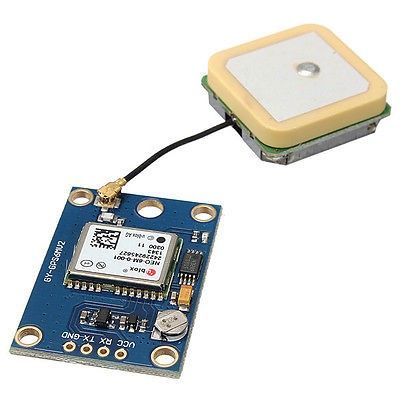
\includegraphics[scale=0.4]{./assets/NEO6M}
		\caption{Modul GPS NEO-6M}
	\end{figure}
	\captionof{table}{Spesifikasi DOIT-ESP32-DEVKIT}
	\begin{longtable}{|p{2cm}|p{8cm}|}
		\hline
		\textit{Time to first fix}&27 detik \textit{cold start}, 27 detik \textit{warm start}, 1 detik \textit{hot start}\\
		\hline
		Sensitivitas&-161dBm \textit{(tracking and navigation)}, -160dBm \textit{(reacquisition)}, -147dBm \textit{(cold start)}, -156dBm \textit{(hot start)}.\\
		\hline
		Akurasi posisi horizontal&2.5m\\
		\hline
		Masukan tegangan&2.7V - 3.6V\\
		\hline
		Maksimum arus&67mA\\
		\hline
		Temperatur operasi&-40\textdegree C - 85\textdegree C\\
		\hline
	\end{longtable}
	\item \textit{Power supply} yang digunakan pada \textit{Sender node} dan \textit{Flying receiver} node menggunakan sebuah linear regulator LM7805 yang dihubungkan pada sebuah baterai LiPo 2S 7.4V, sehingga menghasilkan tegangan keluaran 5V.
	
	\item MJX Bugs 5W\newline Pada perancangan sistem, drone ini digunakan untuk membawa board ESP32 dan modul GPS sebagai node \textit{sender}.
	\begin{figure}[H]
		\centering
		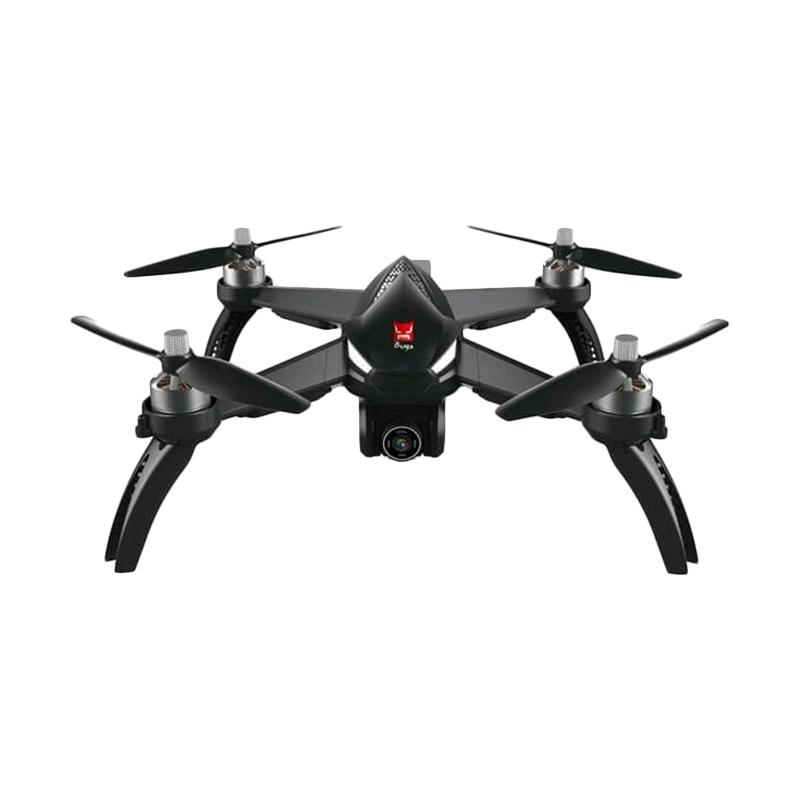
\includegraphics[scale=0.2]{./assets/MJX}
		\caption{Drone MJX Bugs 5W}
	\end{figure}
	\captionof{table}{Spesifikasi drone MJX Bugs 5W}
	\begin{longtable}{|p{3cm}|p{7cm}|}
		\hline
		Frekuensi Remote Control&2.4GHz\\
		\hline
		Baterai drone&7.4V 2S 1800mAh\\
		\hline
		Jarak Remote Control&300-500m\\
		\hline
		Motor&1800KV BLDC\\
		\hline
		ESC&6A Brushless\\
		\hline
	\end{longtable}
\end{enumerate}

\section{Desain Perangkat Lunak}
\subsection{Sender Node}
\begin{figure}[H]
	\centering
	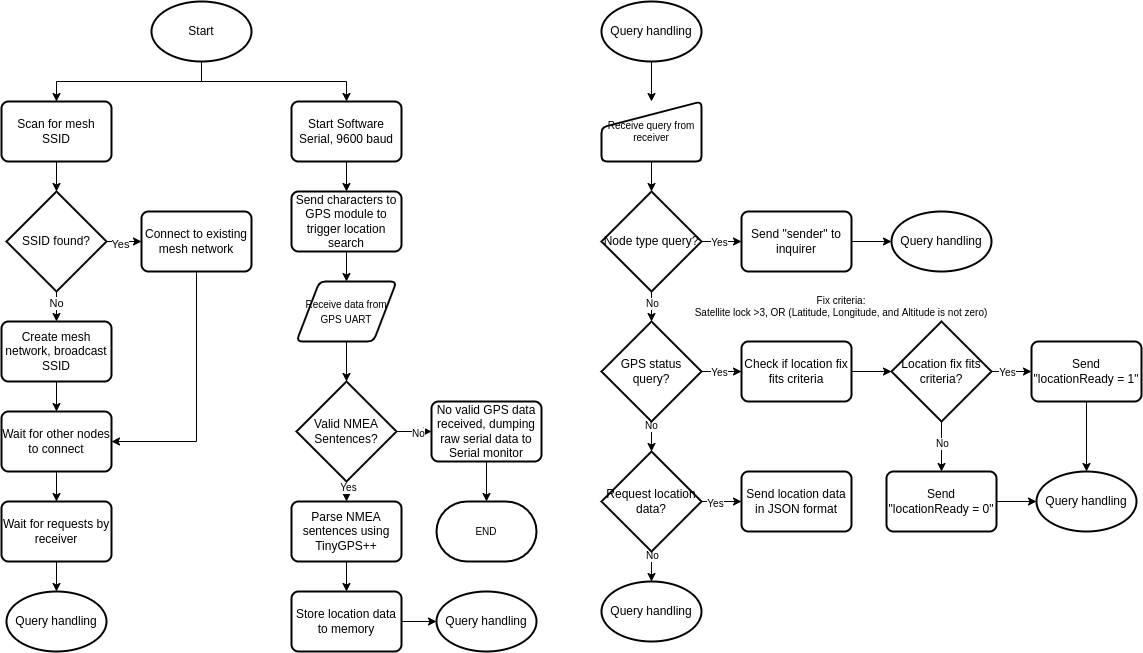
\includegraphics[scale=0.35]{./assets/FlowchartSenderNew}
	\caption{Diagram alur sender node.}
\end{figure}
Gambar 3.6 menunjukkan diagram alur sistem pada node sender. Pada bagian kiri adalah proses inisialisasi sistem, yakni inisialisasi jaringan mesh dan inisialisasi sistem GPS. Pada proses inisialisasi jaringan mesh, board ESP32 melakukan \textit{scanning} terhadap SSID jaringan mesh yang sudah ditetapkan, dan jika ditemukan akan mencoba bergabung dalam jaringan mesh tersebut. Jika SSID tidak ditemukan, maka board ESP32 akan membuat jaringan mesh tersebut dengan sendirinya. Setelah inisialisasi jaringan sudah selesai, maka board ESP32 akan menunggu koneksi dari node lain serta menunggu permintaan dari sebuah node receiver.

Untuk proses inisialisasi GPS, board ESP32 memulai sebuah koneksi serial UART dengan modul GPS NEO-6M menggunakan \textit{library} Software Serial dengan baud rate 9600 bps. Modul GPS NEO-6M membutuhkan sebuah input konstan dari koneksi UART, oleh karena itu board ESP32 secara terus-menerus mengirimkan karakter kepada modul GPS tersebut. Terdapat waktu tunggu lima detik untuk menunggu respon dari modul GPS, jika tidak ada input dari modul GPS setelah lima detik sejak board pertama dinyalakan, maka board akan menghentikan eksekusi program dan menampilkan data mentah dari pin RX di Serial Monitor. Sedangkan jika modul GPS berhasil mengirimkan data melalui UART, maka eksekusi program diteruskan, dan data dari modul GPS tersebut yang berupa kalimat-kalimat NMEA akan ditafsirkan menggunakan \textit{library} TinyGPS++ untuk mendapatkan data lokasi yang kemudian disimpan dalam memori.

Setelah proses inisialisasi sistem selesai, maka board ESP32 akan menunggu permintaan dari node receiver. Terdapat tiga jenis permintaan/\textit{query} yang diterima oleh node sender, yaitu:
\begin{enumerate}
	\item \textit{Node Type Query}\newline \textit{Query} ini merupakan sebuah permintaan dari node receiver yang menanyakan tipe node apa yang telah terhubung dalam jaringan mesh, menggunakan pesan dengan "type" bernilai 1. Respon dari \textit{query} ini untuk node sender adalah mengirimkan sebuah pesan JSON dengan \textit{key} "nodeType" dan \textit{value} "sender".
	\item \textit{GPS Status Query}\newline \textit{Query} ini adalah permintaan dari node receiver untuk mengecek status GPS node sender dan kesiapan node sender untuk mengirimkan data lokasi, dengan menggunakan pesan yang bertipe senilai 2. Kriteria kesiapan tersebut adalah jumlah satelit yang sudah \textit{fix} $\geq$ 3; atau nilai lintang, bujur, dan ketinggian tidak nol. Node sender akan mengirimkan sebuah pesan JSON dengan \textit{key} "locationReady" dan \textit{value} 0 jika kriteria kesiapan GPS belum terpenuhi, dan 1 jika kriteria sudah terpenuhi.
	\item \textit{Request Location Query}\newline \textit{Query} ini adalah permintaan data lokasi dari node receiver menggunakan pesan bertipe senilai 3. Node sender akan mengirimkan sebuah pesan JSON dengan key \textit{latitude, longitude, altitude}, dan \textit{satellite}, berdasarkan data yang sudah didapatkan dari modul GPS.
\end{enumerate}
Node sender juga menerima permintaan pengecekan \textit{round-trip delay} dari node receiver yang menggunakan fungsi \verb|startDelayMeas()|. Fungsi tersebut juga digunakan untuk pengujian \textit{packet loss}.

\subsection{Flying Receiver Node}
\begin{figure}[H]
	\centering
	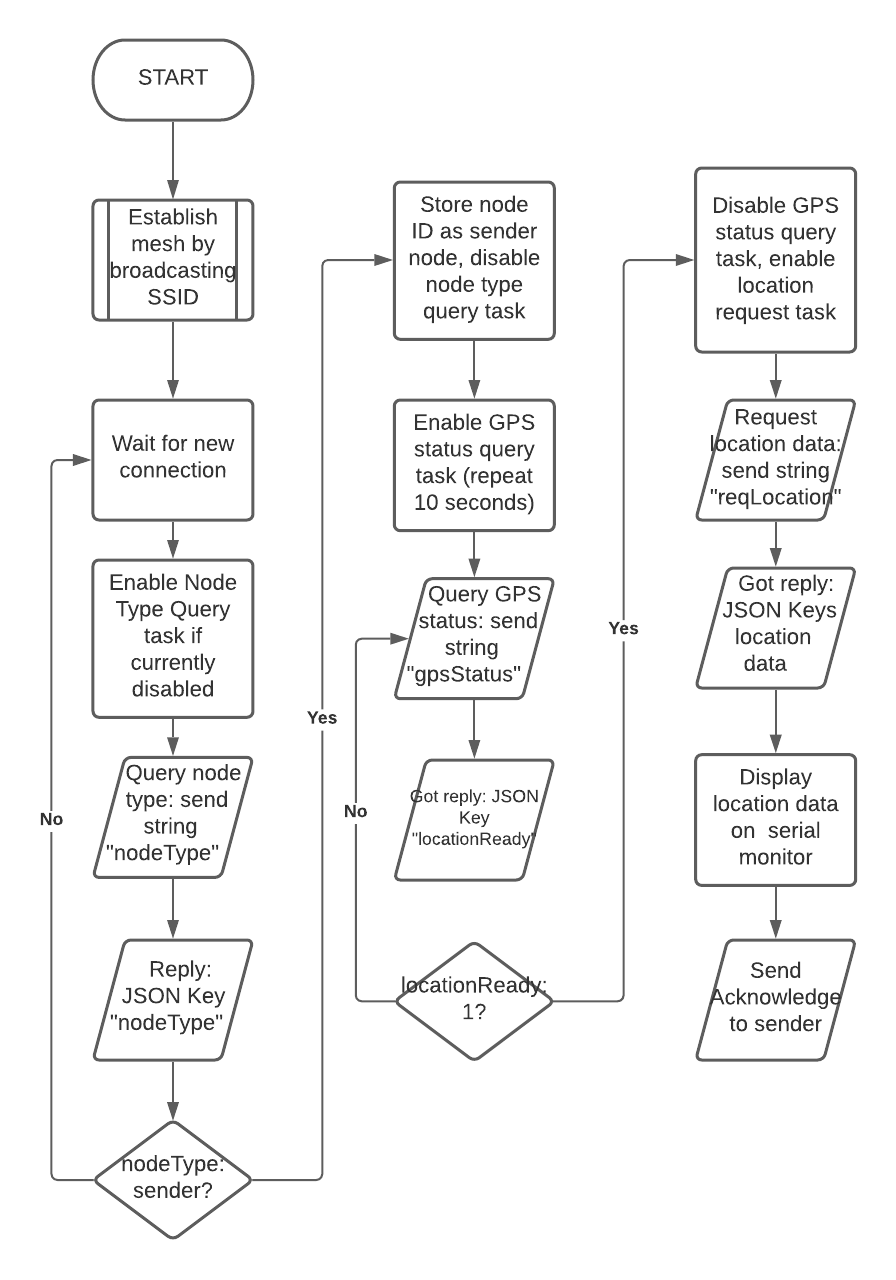
\includegraphics[scale=0.6]{./assets/FlowchartReceiver}
	\caption{Diagram alur node flying receiver, program penarikan data lokasi dari node sender.}
\end{figure}
Flying receiver node adalah node ESP32 yang diterbangkan menggunakan sebuah drone yang bertugas menerima data lokasi dari sender node, menguji kinerja jaringan terbang, sekaligus mencatat ke sebuah kartu memori MicroSD. Tugas-tugas tersebut dibagi menjadi dua program pada satu node, yaitu program pertama yang menarik data lokasi dari sender node, dan program kedua yang menguji kinerja jaringan setelah selesainya pelaksanaan program pertama.

Pelaksanaan masing-masing task pada node ini terjadwal menggunakan fitur \textit{Task Scheduler}, dan dilaksanakan secara berurutan, yakni melakukan koneksi pada jaringan mesh, melakukan \textit{query} tipe node-node lainnya pada jaringan, melakukan \textit{query} kondisi GPS pada node sender, dan melakukan \textit{query} data lokasi dari sender node.

\begin{figure}[H]
	\centering
	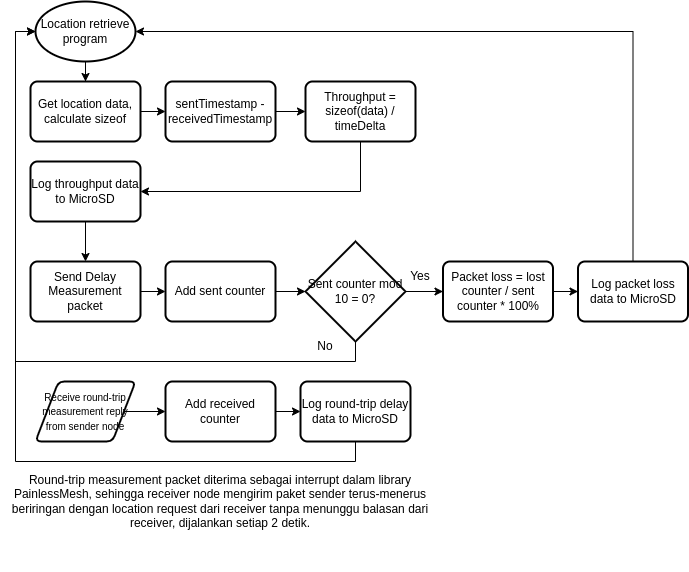
\includegraphics[scale=0.5]{./assets/FlowchartNetworkTestNew}
	\caption{Diagram alur node flying receiver, program pengujian jaringan.}
\end{figure}

Berdasarkan yang dipaparkan pada Bab 2, pengujian kinerja jaringan yang dilakukan adalah pengujian \textit{throughput}, \textit{round-trip delay}, dan \textit{packet loss}.
\begin{enumerate}
	\item \textit{Throughput}\newline Pengujian \textit{throughput} dilakukan bersamaan dengan program penarikan data lokasi, yakni dengan menghitung besar paket data lokasi yang dikirim, membandingkan waktu pengiriman dan waktu penerimaan paket data, lalu membagi besar paket data tersebut dengan selisih waktu pengiriman dan penerimaan paket data.
	\newline Misalkan dengan paket data sebesar 12 byte, waktu pengiriman paket data dari \textit{sender} senilai 1000 ms, dan waktu penerimaan paket data di \textit{receiver} senilai 1250 ms, maka nilai \textit{throughput} sebesar:
	\begin{equation}
		\begin{aligned}
		Throughput &= \frac{sizeof(packet)}{t_1 - t_0}\\
		&= \frac{12}{1250 - 1000}\\
		&= \frac{12}{250} \\
		& = 0.048 B/ms \\
		& = 48 B/s
		\end{aligned}
	\end{equation}
	\item \textit{Round-trip delay}\newline Pengujian \textit{round-trip delay} menggunakan fungsi \verb|startdelayMeas()| pada library PainlessMesh yang menghasilkan \textit{return value} sebesar nilai \textit{delay} dalam mikrosekon. \textit{Receiver node} melakukan tes ini tepat setelah menerima data lokasi dari \textit{sender node} dengan memanggil fungsi \verb|startDelayMeas()|. Setelah fungsi tersebut dipanggil, maka \textit{receiver} menambahkan jumlah \textit{counter} untuk paket data yang dikirim.
	\newline Pada sistem ini, $t_0$ adalah \textit{timestamp internal clock} board ESP32 saat permintaan pengukuran \textit{delay} dibuat oleh \textit{receiver} node, $t_1$ adalah \textit{timestamp} jaringan saat permintaan pengukuran \textit{delay} diterima oleh \textit{sender} node, $t_2$ adalah \textit{timestamp} jaringan saat balasan dari \textit{sender} node dibuat, dan $t_3$ adalah \textit{timestamp internal clock} board ESP32 saat balasan pengukuran \textit{delay} diterima oleh \textit{receiver} node. Misalkan nilai $t_0$ = 20000 $\mu$s, $t_1$ = 25000 $\mu$s, $t_2$ = 35000 $\mu$s, dan $t_3$ = 60000 $\mu$s:
	\begin{equation}
		\begin{aligned}
			t_{roundtrip} &= (t_3 - t_0) - (t_2 - t_1)\\
			&= (60000 - 20000) - (35000 - 25000)\\
			&= 40000 - 10000\\
			&= 30000 \mu S\\
			&= 30 ms
		\end{aligned}
	\end{equation}
	\item \textit{Packet loss}\newline Pengujian \textit{packet loss} dilakukan setelah 10 kali \textit{receiver} mengirim paket data lalu membandingkan berapa kali fungsi \verb|startdelayMeas()| dipanggil terhadap jumlah paket balasan dari \textit{sender} node.
	\newline Misalkan telah dikirimkan 80 paket pengukuran \textit{delay} dan telah diterima 75 paket respon pengukuran \textit{delay}, maka:
	\begin{equation}
		\begin{aligned}
			Packet Loss &= (1-\frac{ack_{RX}}{p_{TX}})\times 100\% \\
			&= (1 - \frac{75}{80}) \times 100 \% \\
			&= 0.0625 \times 100 \% \\
			&= 6.25 \%
		\end{aligned}
	\end{equation}
	\item \textit{Signal strength}\newline Pendataan \textit{signal strength} dilakukan setiap kali ada permintaan data dari receiver, menggunakan fungsi \verb|WiFi.RSSI()| dari ESP32.
\end{enumerate}